\documentclass[11pt]{exam}
\newcommand{\myname}{Sihao Yin, Yuxuan Jiang} %Write your name in here

\newcommand{\myUCO}{0028234022, 0028440468} %write your UCO in here

\newcommand{\myhwtype}{Homework}
\newcommand{\myhwnum}{1} %Homework set number
\newcommand{\myclass}{CS580}
\newcommand{\mylecture}{}
\newcommand{\mysection}{}
\usepackage{listings}
% Prefix for numedquestion's
\newcommand{\questiontype}{Question}

% Use this if your "written" questions are all under one section
% For example, if the homework handout has Section 5: Written Questions
% and all questions are 5.1, 5.2, 5.3, etc. set this to 5
% Use for 0 no prefix. Redefine as needed per-question.
\newcommand{\writtensection}{0}

\usepackage{amsmath, amsfonts, amsthm, amssymb}  % Some math symbols
\usepackage{enumerate}
\usepackage{enumitem}
\usepackage{graphicx}
\usepackage{hyperref}
\usepackage[all]{xy}
\usepackage{wrapfig}
\usepackage{fancyvrb}
\usepackage[T1]{fontenc}
\usepackage{listings}

\usepackage{centernot}
\usepackage{mathtools}
\DeclarePairedDelimiter{\ceil}{\lceil}{\rceil}
\DeclarePairedDelimiter{\floor}{\lfloor}{\rfloor}
\DeclarePairedDelimiter{\card}{\vert}{\vert}


\setlength{\parindent}{0pt}
\setlength{\parskip}{5pt plus 1pt}
\pagestyle{empty}

\def\indented#1{\list{}{}\item[]}
\let\indented=\endlist

\newcounter{questionCounter}
\newcounter{partCounter}[questionCounter]

\newenvironment{namedquestion}[1][\arabic{questionCounter}]{%
    \addtocounter{questionCounter}{1}%
    \setcounter{partCounter}{0}%
    \vspace{.2in}%
        \noindent{\bf #1}%
    \vspace{0.3em} \hrule \vspace{.1in}%
}{}

\newenvironment{numedquestion}[0]{%
	\stepcounter{questionCounter}%
    \vspace{.2in}%
        \ifx\writtensection\undefined
        \noindent{\bf \questiontype \; \arabic{questionCounter}. }%
        \else
          \if\writtensection0
          \noindent{\bf \questiontype \; \arabic{questionCounter}. }%
          \else
          \noindent{\bf \questiontype \; \writtensection.\arabic{questionCounter} }%
        \fi
    \vspace{0.3em} \hrule \vspace{.1in}%
}{}

\newenvironment{alphaparts}[0]{%
  \begin{enumerate}[label=\textbf{(\alph*)}]
}{\end{enumerate}}

\newenvironment{arabicparts}[0]{%
  \begin{enumerate}[label=\textbf{\arabic{questionCounter}.\arabic*})]
}{\end{enumerate}}

\newenvironment{questionpart}[0]{%
  \item
}{}

\newcommand{\answerbox}[1]{
\begin{framed}
\vspace{#1}
\end{framed}}

\pagestyle{head}

\headrule
\header{\textbf{\myclass\ \mylecture\mysection}}%
{\textbf{\myname\ (\myUCO)}}%
{\textbf{\myhwtype\ \myhwnum}}

\begin{document}
\thispagestyle{plain}
\begin{center}
  {\Large \myclass{} \myhwtype{} \myhwnum} \\
  \myname{} (\myUCO{}) \\
  \today
\end{center}


%Here you can enter answers to homework questions

\begin{numedquestion}
  \begin{enumerate}
      \item The following is how the recursion tree would look like \\
       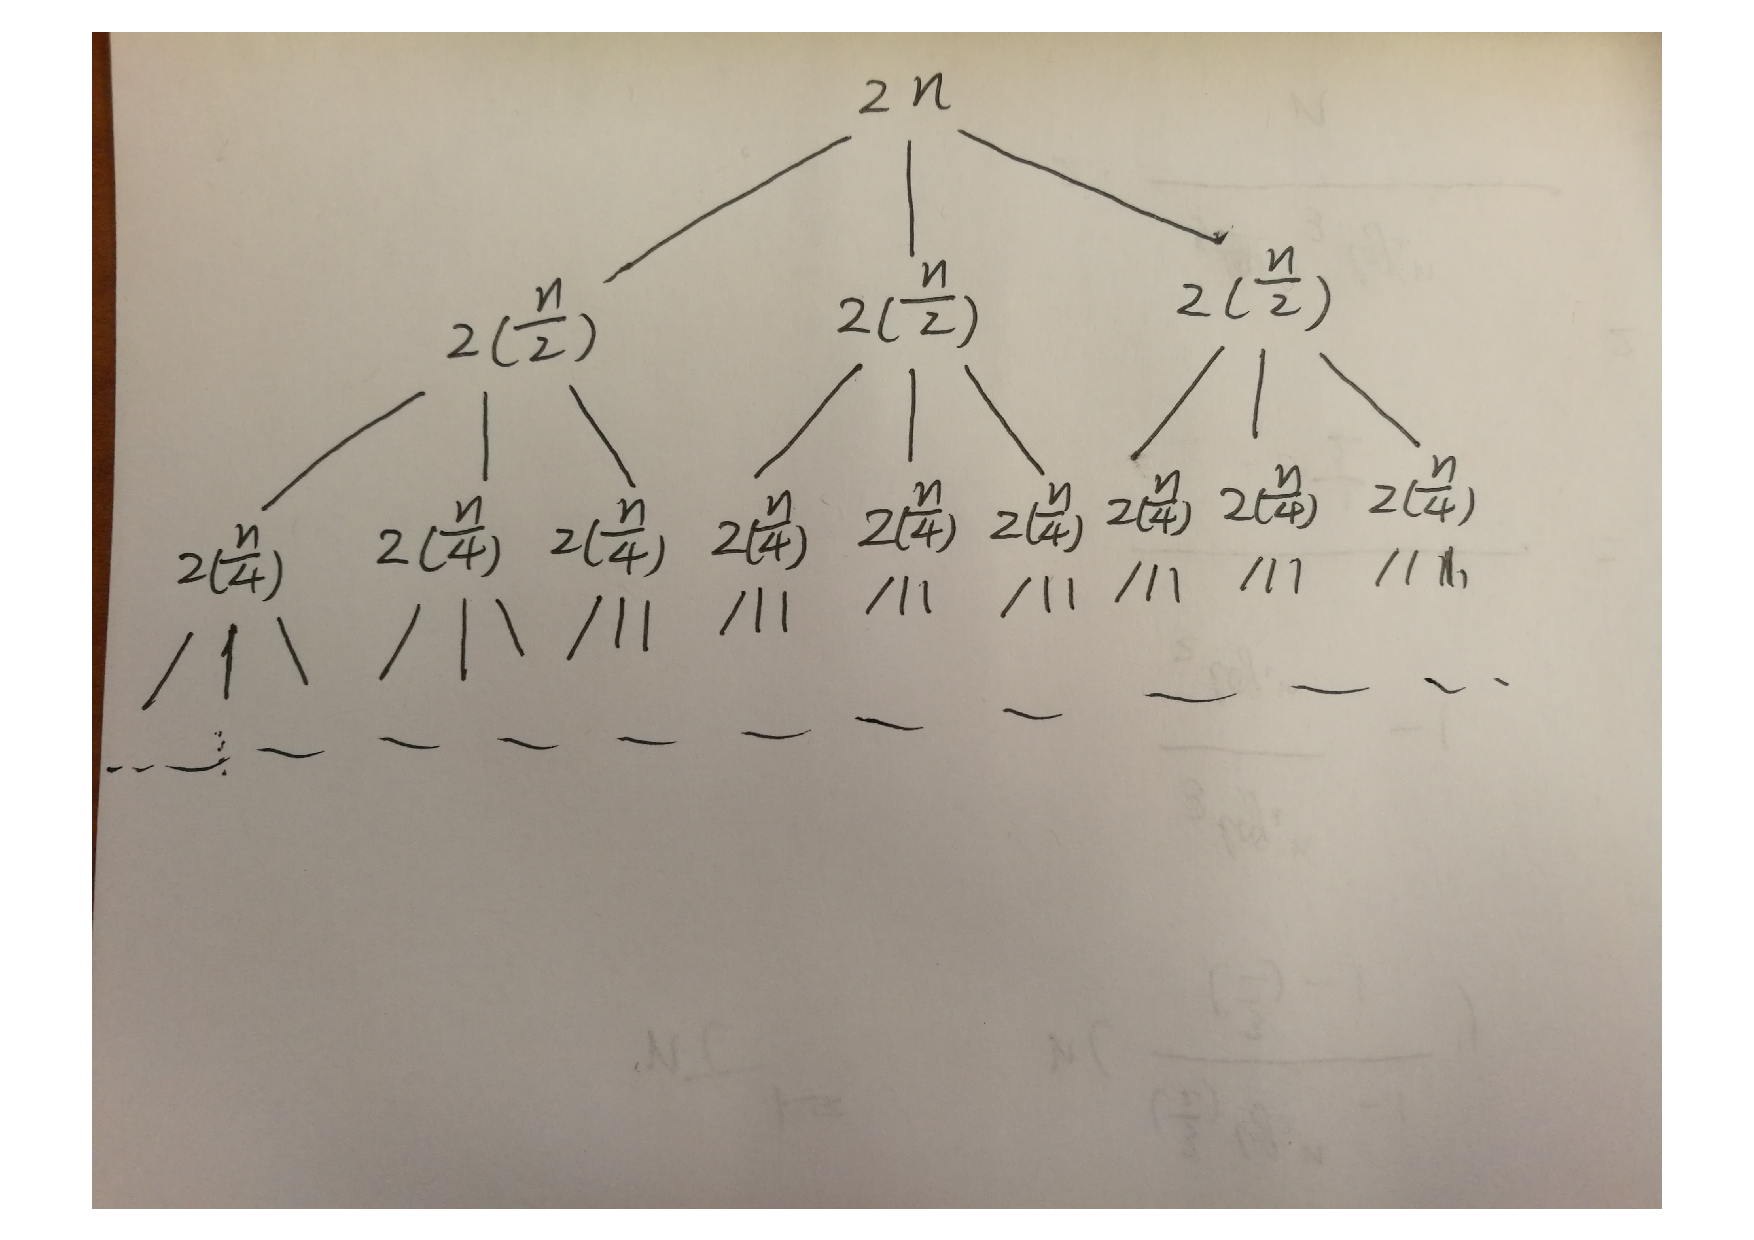
\includegraphics[scale=0.5]{images/fig1.pdf}
     
      Sum of second level: 3 * 2($\frac{n}{2}$) = 3n \\
      Sum of third level: 9 * 2($\frac{n}{4}$) = $\frac{9}{2}$n \\
      Sum of fourth level: 27 * 2($\frac{n}{8}$) = $\frac{27}{4}$n \\\\
      Since we are dividing by 2, the height of the recursion tree will be $log_2^n$\\
      Since the number of nodes at height k is $3^k$, the number of nodes at the base level is $3^{log_2^n}$.
      Hence T(n) = 2n + 2 * $\frac{3}{2}$ n + 2 * $(\frac{3}{2})^2$n + 2 * $(\frac{3}{2})^3$n + ...+
                    2 * $(\frac{3}{2})^{log_2^n - 1}$n + $6*3^{log_2^n}$\\
                 = 2 * (n + $\frac{3}{2}$ n + $(\frac{3}{2})^2$n + $(\frac{3}{2})^3$n + ... + $(\frac{3}{2})^{log_2^n-1}$n) + $6*n^{log_2^3}$\\\\
     Since n + $\frac{3}{2}$ n + $(\frac{3}{2})^2$n + $(\frac{3}{2})^3$n +...+ $(\frac{3}{2})^{log_2^n-1}$n is a geometric series, with a = n and r = $\frac{3}{2}$, the sum of it will be 
     $\sum_{k=0}^{log_2^n-1}$ n*($(\frac{3}{2})^k$) = n * $\frac{(\frac{3}{2})^{log_2^n}-1}{(\frac{3}{2})-1}$ = 2n * $(
     (\frac{3}{2})^{log_2^n}-1)$
     = $2(n^{log_2^3})-2n$\\\\
     
     Hence T(n) = 4*$(n^{log_2^3})-4n + 6*n^{log_2^3}$ = $\Theta$($n^{log_2^3}$)
     \pagebreak
     
     
      \item The following is how the recursion tree would look like \\
      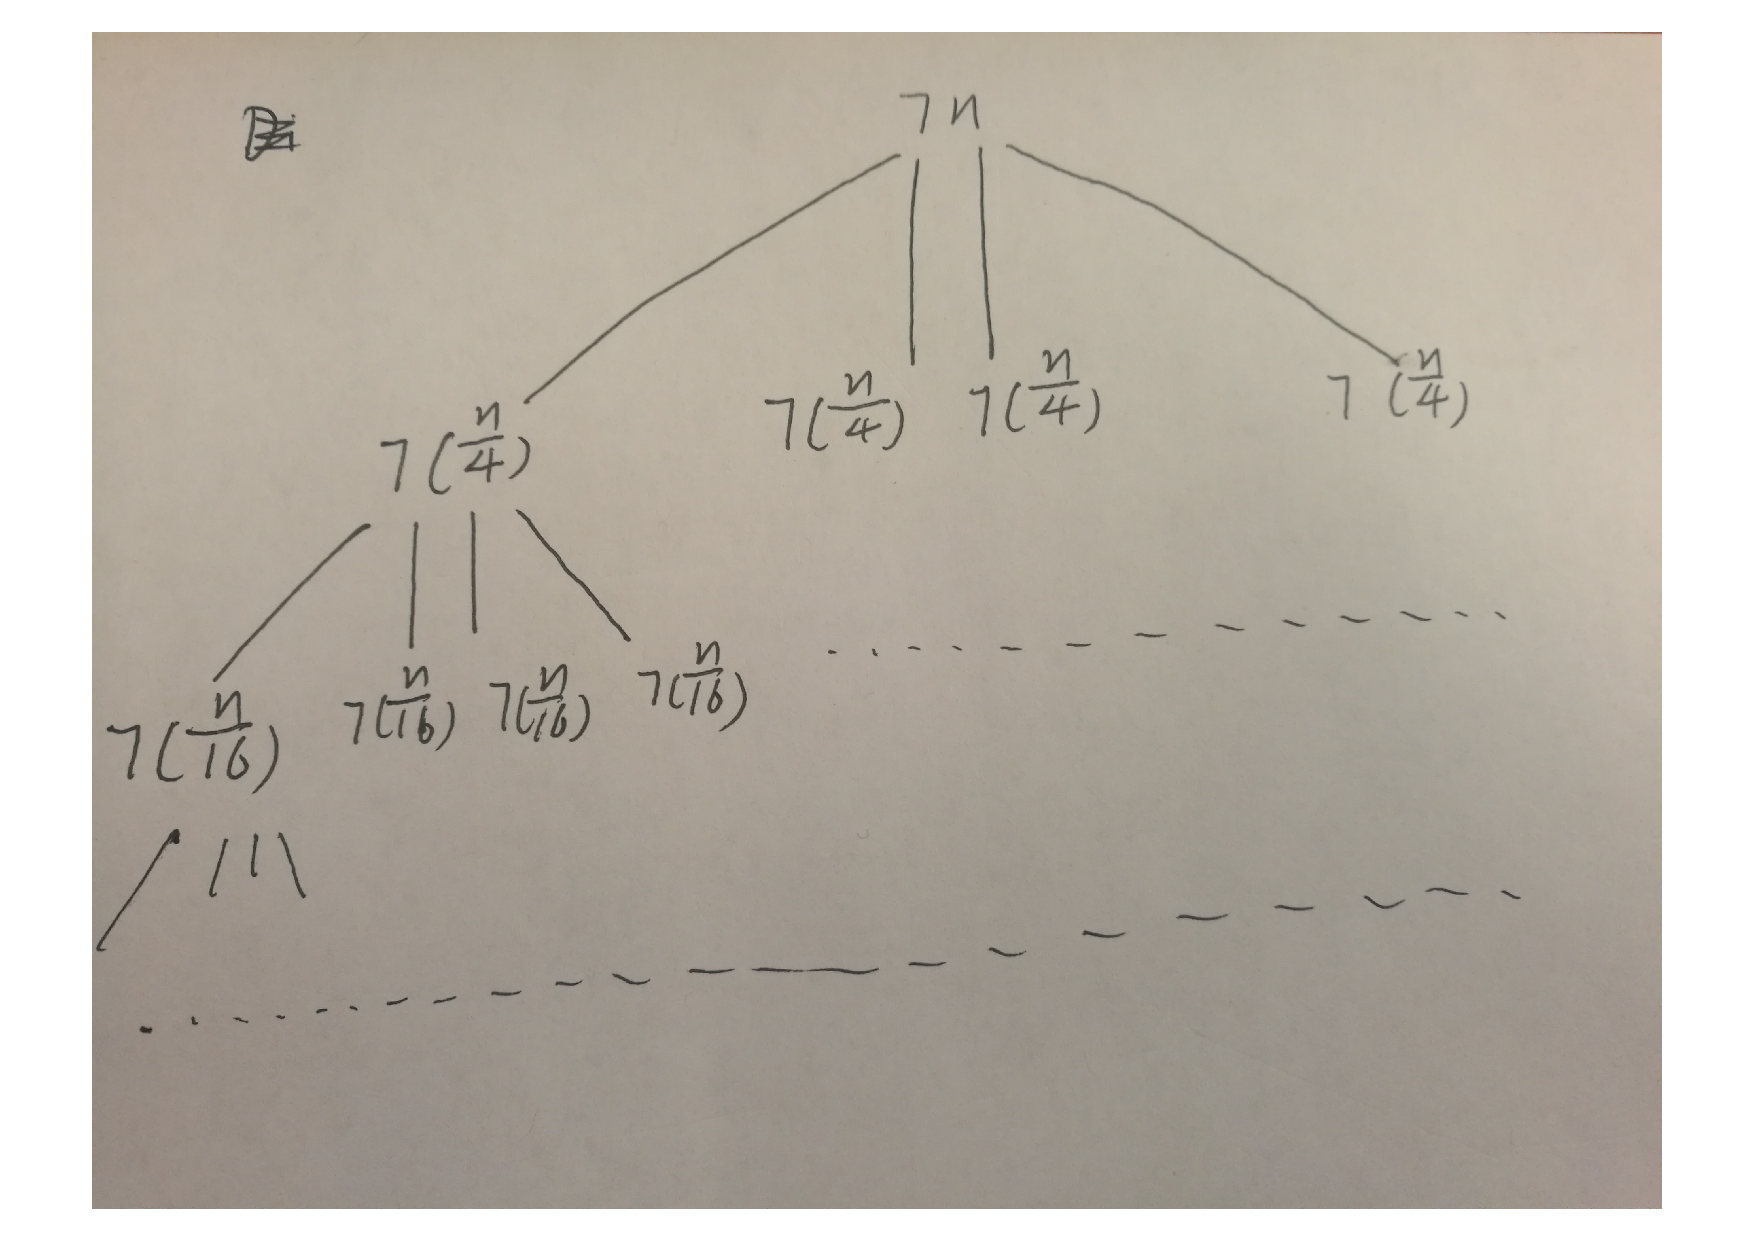
\includegraphics[scale=0.5]{images/fig2.pdf}
      
      Sum of the second level: 7*(4 * $\frac{n}{4}$) \\
      Sum of the third level: 7*($4^2$ * $\frac{n}{4^2}$) \\
      Sum of the fourth level: 7*($4^3$ * $\frac{n}{4^3}$) \\\\
      
      Since we are dividing by 4, the height of the tree will be $log_4^n$ \\
      Since the number of nodes at height k is $4^k$, the number of nodes at the base level is $4^{log_4^n}$ = n.\\
      Hence T(n) = 7n + 7n +....+7n \\
                 = 7n * ($log_4^n$)
                 = 7n * $\frac{1}{2}* log_2^n$\\\\
                
     
     Hence T(n) = 7n * $\frac{1}{2}* log_2^n$ = $\Theta$($n*{log_2^n}$)
     \pagebreak
     \item The following is how the recursion tree would look like\\
     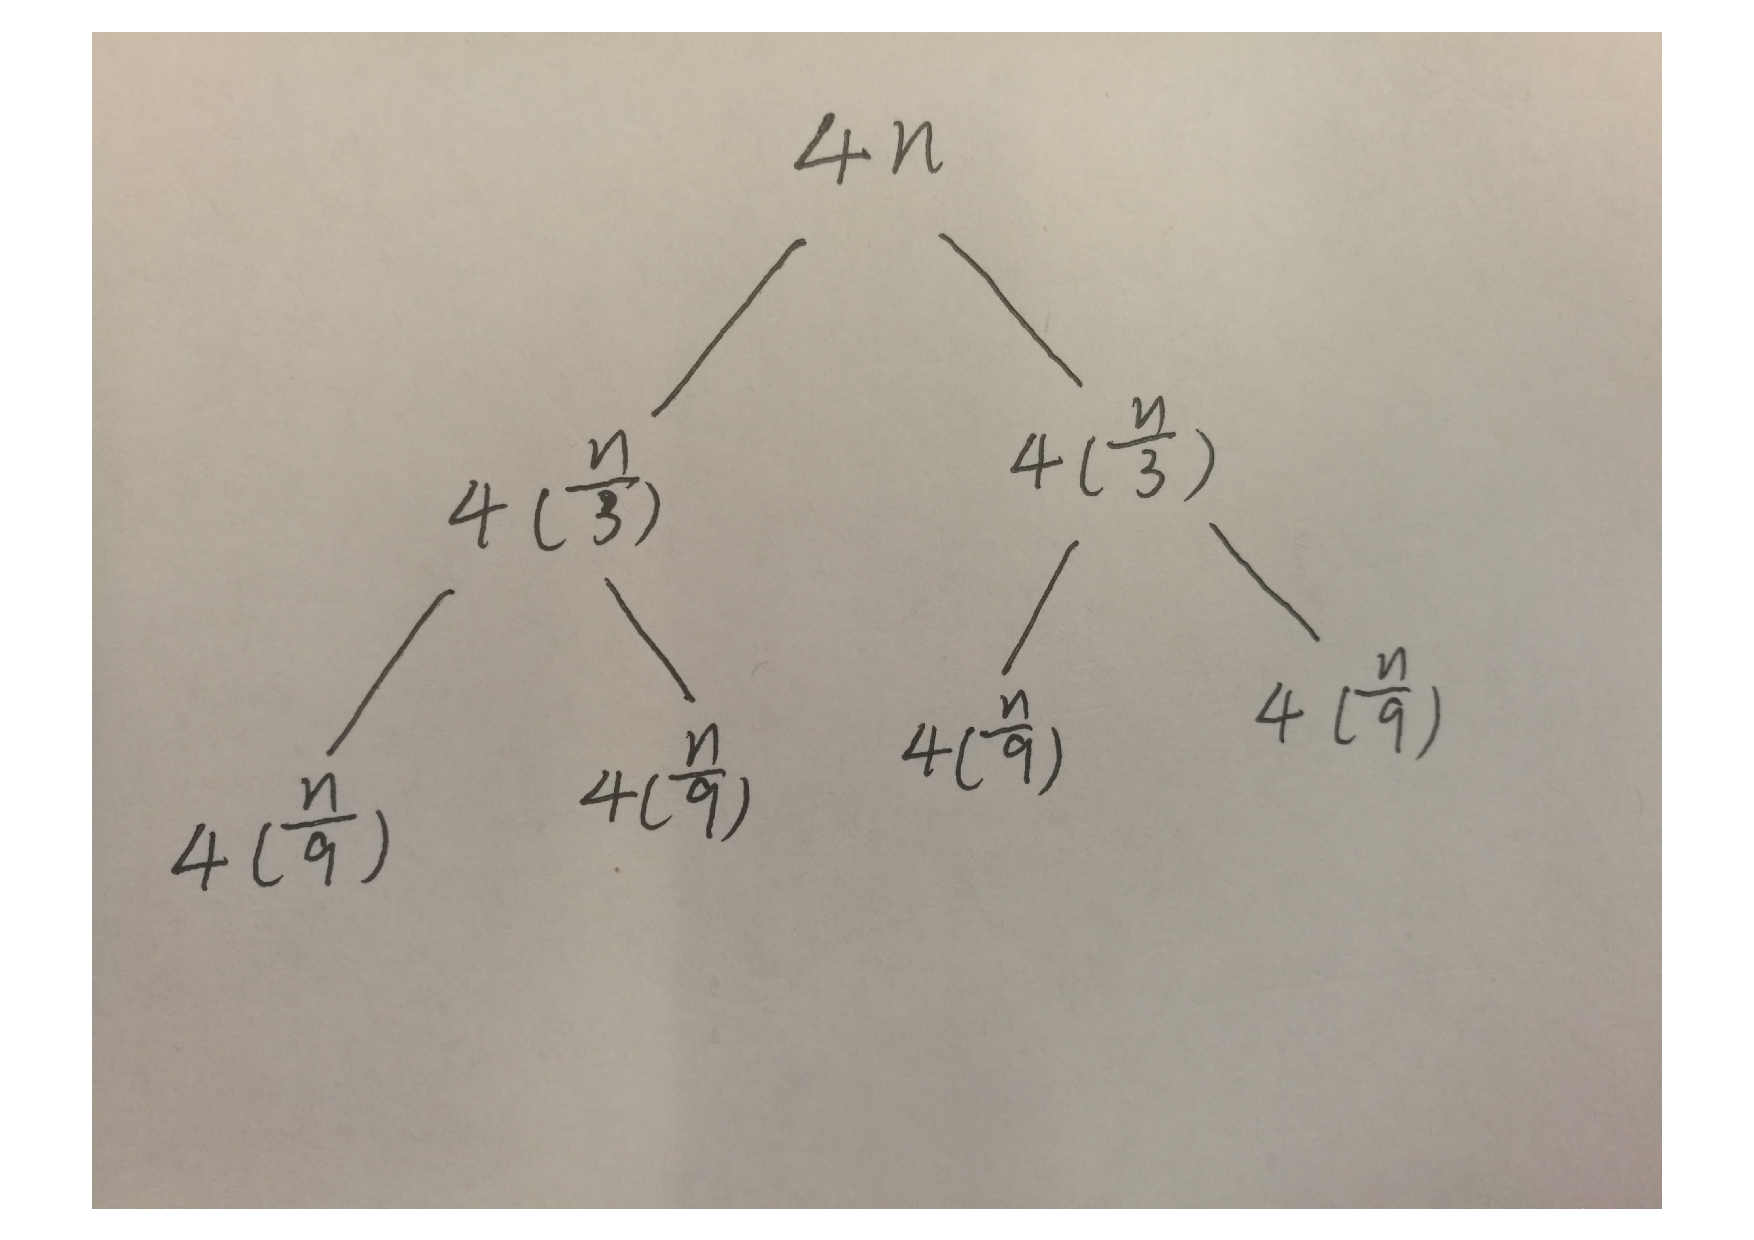
\includegraphics[scale=0.5]{images/fig3.pdf}
       
     Sum of the second level: 4*(2 * $\frac{n}{3}$)\\
     Sum of the third level: 4*($2^2$ *$\frac{n}{3^2}$) \\
     Sum of the fourth level: 4*($2^3$ * $\frac{n}{3^3}$) \\\\
     Since we are diving by 3, the height of the recursion tree will be $log_3^n$ \\
     Since the number of nodes at height k is $2^k$, the number of nodes at the base level is $2^{log_3^n}$.\\
     Hence T(n) = 4n + 4 * $\frac{2}{3}$ n + 4 * $(\frac{2}{3})^2$n + 4 * $(\frac{2}{3})^3$n + ...+
                    4 * $(\frac{2}{3})^{log_3^n}$n + $2^{log_3^n-1}$\\
                 = 4 * (n + $\frac{2}{3}$ n + $(\frac{2}{3})^2$n + $(\frac{2}{3})^3$n + ... + $(\frac{2}{3})^{log_3^n-1}$n) + $n^{log_3^2}$ \\\\
     Since n + $\frac{2}{3}$ n + $(\frac{2}{3})^2$n + $(\frac{2}{3})^3$n +...+ $(\frac{2}{3})^{log_3^n}$n is a geometric series, with a = n and r = $\frac{2}{3}$, the sum of it will be 
     $\sum_{k=0}^{log_3^n-1}$ n*($(\frac{2}{3})^k$) = n * $\frac{1-(\frac{2}{3})^{log_3^n}}{(1-\frac{2}{3})}$ = $3n-3(n^{log_3^2})$ \\\\
     
     Hence T(n) = $4 * (3n-3(n^{log_3^2})) + n^{log_3^2}$ = $12n-11(n^{log_3^2})$= $\Theta$(n)\\\\
  \end{enumerate}
\end{numedquestion}

\pagebreak
\begin{numedquestion}
  Below is the pseudocode, we keep a global counter for number of inversions. This is essentially merge sort\\\\
    \begin{lstlisting}
     
     numOfInver = 0
     function mergeSort(A[1...N]):
        if N > 1:
            m = floor(N/2)
            mergeSort(A[1...m])
            mergeSort(A[m+1...N])
            merge(A[1...N],m)
 
     function merge(A[1...N],m):
	    B = a new array with length equals to left.length+right.length
	    i = 1
	    j = m+1
	    for k from 1 to N:
	        if j > N:
	            B[k] = A[i]
	            i = i + 1
	       else if i > m:
	            B[k] = A[j]
	            j = j + 1
	       else if A[i] <= A[j]:
	            B[k] = A[i]
	            i = i + 1
	       else:
	            numOfInver = numOfInver + (j-m)
	            j = j + 1
	   
	   for k from 1 to N:
	       A[k] = B[k]
	   
	   return B

    \end{lstlisting}

\textbf{Analysis:} 
\begin{enumerate}
    \item this algorithm is correct because in merge sort, the two subarrays are sorted when merging. Hence, when we check if A[i] > A[j], such an ith element must be on the left subarray, and jth element must be on the right. Since the right subarray is sorted, the ith element is also larger than any elements on the right subarray which are smaller than the jth element. Hence, numOfInver = numOfInver + (j-m)
    \item In function mergesort, we divide the input array in half and recursively call the function mergesort for each half. Then we call the function merge to merge the two halves. 
    \item In function merge, we loop through the two input arrays and increment the inversion counter accordingly. This takes linear time 
    \item With above, we have the this recurrence.: T(n) = 2($\frac{n}{2}$) + O(n).  
    \item We solve this recursion using the recursion tree method \\
    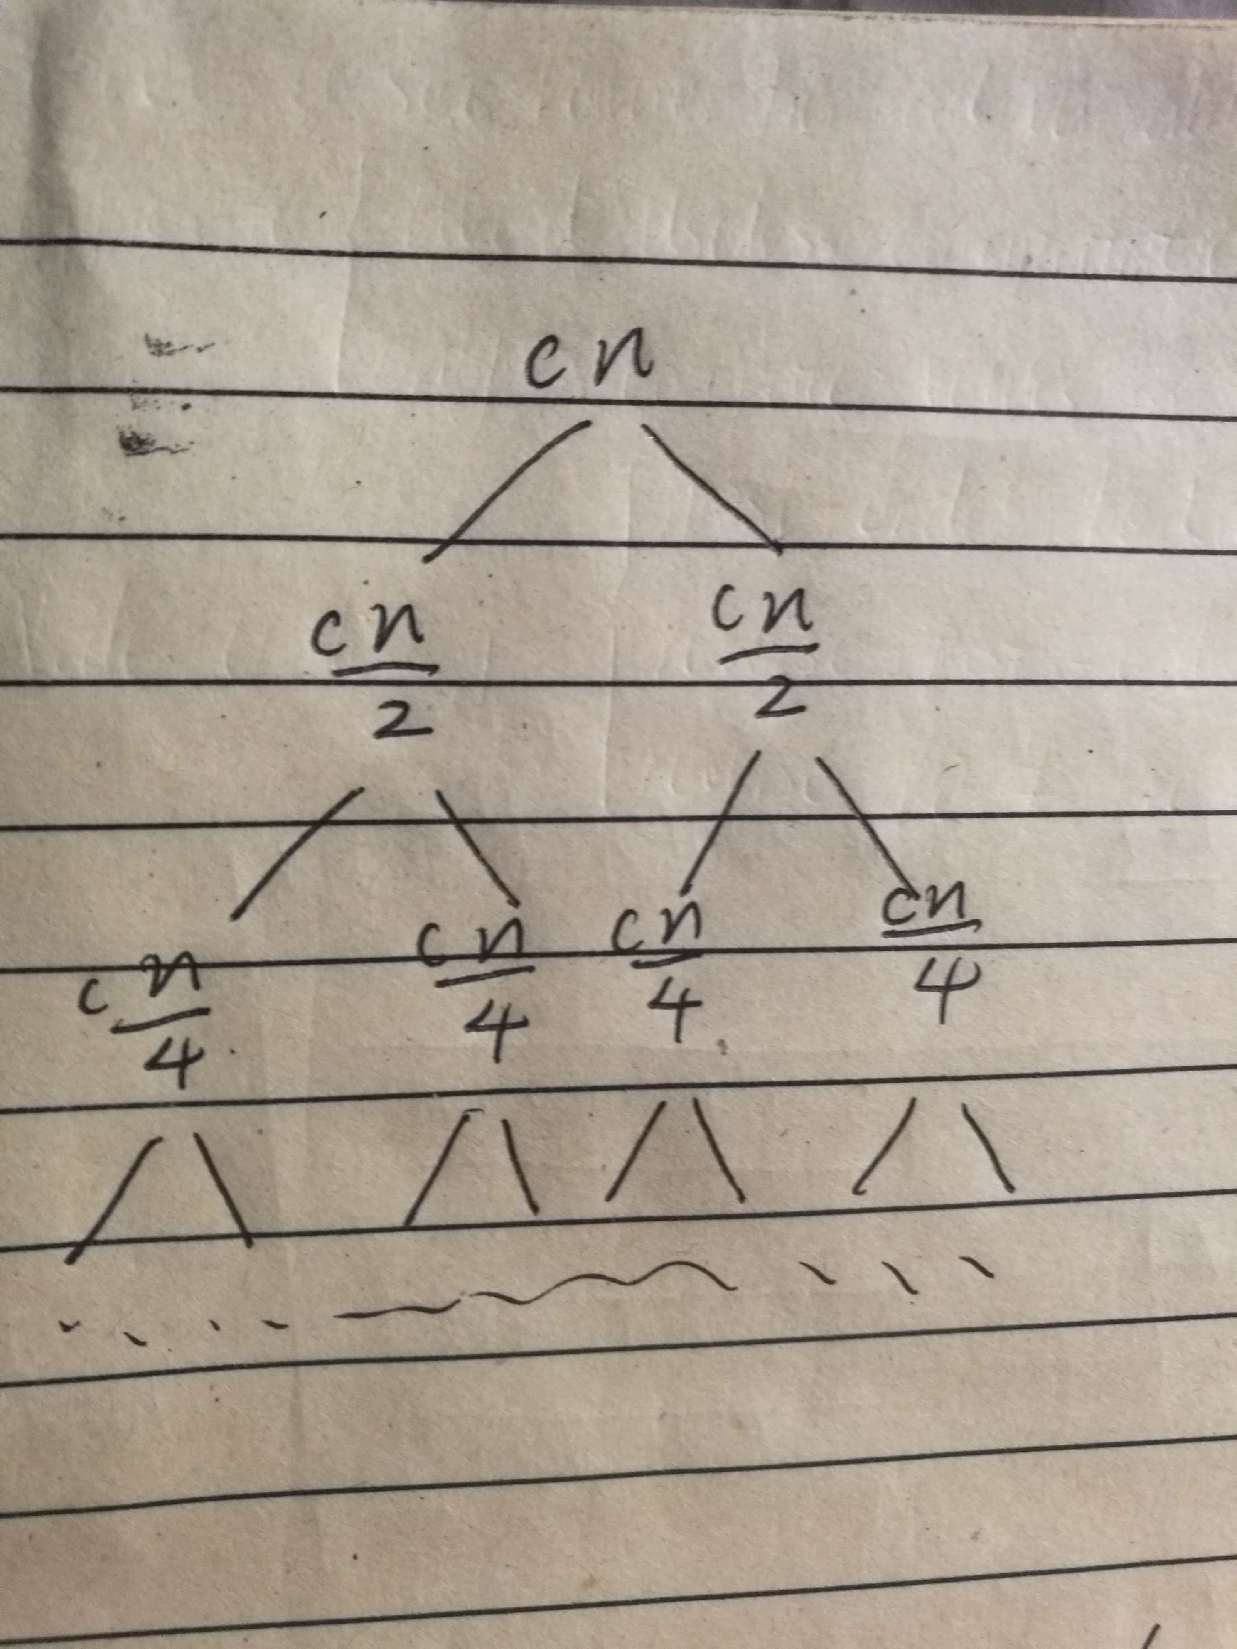
\includegraphics[scale=0.5]{images/merge.pdf}
        \begin{enumerate}
            \item Sum of the second level: cn
            \item Sum of the third level: cn
            \item Sum of the fourth level: cn
        \end{enumerate}
        Since we are dividing the input array by half each time in mergeSort, the height of the recursion tree is $log_2^n$. Hence T(n) = cn + cn + ... + cn = cn *  $log_2^n$ = O(n $log_2^n$) 
\end{enumerate}
      
\end{numedquestion}


% if you do not solve some of the questions use this command to increment counter
%\setcounter{questionCounter}{4}
%\begin{numedquestion}
%  Questions 2 and 3 were not solved, this is an answer to question 5.
%\end{numedquestion}


% if questions have subparts, use this command
%\pagebreak
%\begin{numedquestion}
%  Use the alphaparts environment to for letters.
%  \begin{alphaparts}
%    \item Part a
%    \item Part b
%    \item Part c
%  \end{alphaparts}
%\end{numedquestion}


%\begin{numedquestion}
%  Using the \texttt{description} environment is a great way to typeset induction proofs!
%  \begin{description}
%    \item[Base Case:]
%      Here I have my base case.
%    \item[Induction Hypothesis:]
%      Assume things to make proof work. 
%    \item[Induction Step:]
%      Prove all the things.
%  \end{description}

%  Therefore, we have proven the claim by induction on in the \texttt{description} environment.
%\end{numedquestion}



\end{document}
